%% This is file 'chapter1.tex'
%% It is included by hhuthesis-example.tex for hhuthesis.
%%
%% Copyright(C) 2020, Wenhan Cao
%% College of Water Conservancy and Hydropower Engineering, Hohai University.
%%
%% Version:v1.0.0
%% Last update: July 19th, 2020.
%%
%% Home Page of the Project: https://github.com/caowenhan/thesis
%%
%% This file may be distributed and / or modified under the conditions of the
%% LaTeX Project Public License, either version 1.3c of this license or (at your
%% option) any later version. The latest version of this license is in:
%%
%% http://www.latex-project.org/lppl.txt
%%
%% and version 1.3c or later is part of all distributions of LaTeX version
%% 2008/05/04 or later.
%%
\chapter{样本章}
\label{chap:sample}
\section{研究的目的和意义}
\label{sec:aim}

水库大坝不仅是调控水资源时空分布、优化水资源配置的重要工程措施,也是江河防洪工程体系的重要组成部分,是经济社会发展不可替代的基础支撑\cite{胡四一2008确保水库大坝安全意义重大任务艰巨}。我国是举世闻名的治水大国,建坝数量、建设规模与技术难度均居世界前列,其中,混凝土坝由于其可靠性高和环境适应能力强等特点,是目前我国大、中型水利工程的主要坝型。然而,由于我国特殊的水电资源分布特征,有相当一部分混凝土坝修建于我国高海拔或高纬度的东北、西北等气候寒冷区域,由于寒冷地区普遍存在昼夜温差大、年平均冰冻周期长和年际冻融次数多等特点,极易导致坝体混凝土材料在严寒气候条件和复杂荷载工况作用下,出现冻融破坏和溶蚀损伤等典型渗水病害问题,进而导致大坝服役性能的衰退,威胁工程服役安全。\par
寒冷地区在地理学领域是指由于高海拔或者高纬度而形成的特别寒冷的气候区域,广义上中国的寒冷地区主要包括整个青藏高原,以及甘肃、内蒙古和新疆的高山地区以及东北和华北部分地区。寒冷地区气候条件十分恶劣,四季气温周期交替变化,气温年变幅大,冰冻期长,导致这些地区水利工程每年需要承受多次冻融循环(我国现场环境年均冻融循环次数分布如图\ref{fig:map}\cite{武海荣2012混凝土冻融环境区划与抗冻性寿命预测}。

\begin{figure}[H]
	\centering
	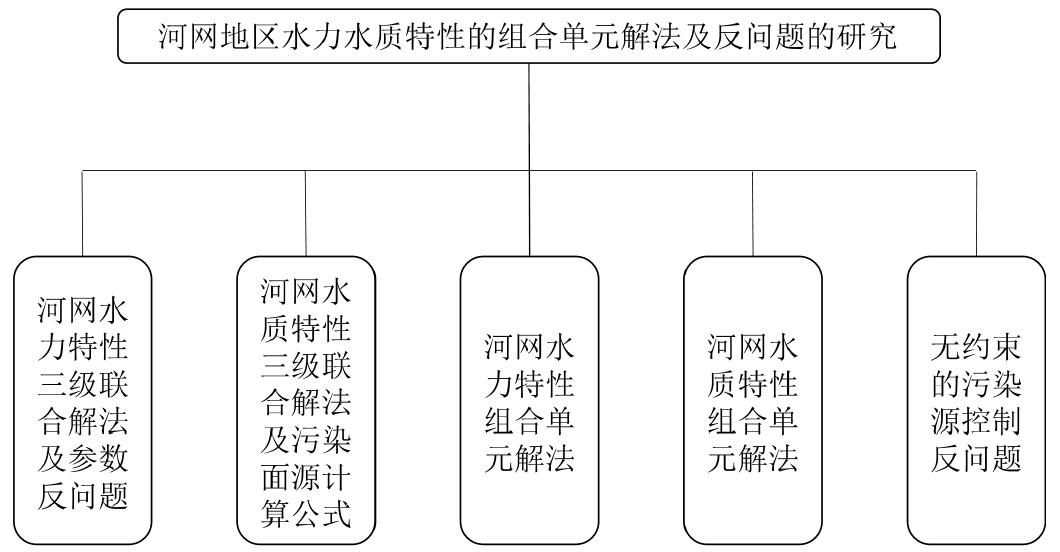
\includegraphics[width=0.75\textwidth]{figure1.jpg}
	\bicaption{我国现场环境年均冻融循环次数分布图}{The average field environmental freezing and thawing times in China}\label{fig:map}
\end{figure}
\section{坝体混凝土材料微观结构特性表征}
本节在对水泥基材料微观尺度基本水化反应和结构特性研究的基础上,引入三维微观水化模型,系统研究坝体混凝土材料三维微观结构特性,从而为后续研究寒冷地区渗水病害影响下坝体混凝土微观力学性能演化特性奠定基础条件。

\subsection{水泥基材料基本水化反应}
硅酸盐水泥生料主要由钙、硅、氧三种化学元素组成的氧化物构成,相应化学成分和简称分别为:\ce{CaO}(C)、\ce{SiO2}(S)、\ce{Al2O3}(A)、\ce{Fe2O3}(F)、\ce{MgO}(M)、\ce{SO3}($\bar{S}$)和\ce{H2O}(H),相应水泥熟料扫描电子显微镜图如图\ref{fig:diagram}。

\begin{figure}[H]
	\centering
	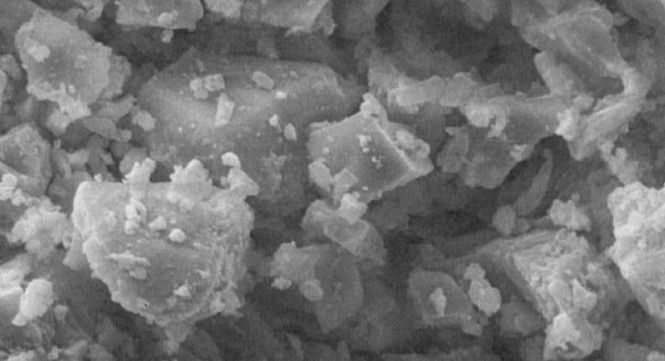
\includegraphics[width=0.75\textwidth]{figure2.jpg}
	\bicaption{硅酸盐水泥熟料颗粒扫描电子显微镜图}{The electron microscope scanning diagram of Portland cement Particle}\label{fig:diagram}
\end{figure}
\subsection{水泥微观水化模型基本原理}
本文主要通过引入HYMOSTRUC 3D模型用于模拟水泥水化反应和水泥基材料微观结构生成。该模型最早由荷兰Technische Universiteit Delft的Klaas van Breugel教授于1991年提出\cite{Delft1991Simulation,钱智炜2010水泥净浆微观结构断裂破坏过程的三维模拟},后经该大学的微观实验室(Microlab)研究人员的开发和完善,逐步形成了比较成熟的水泥微观水化数值计算平台。HYMOSTRUC 3D模型可以综合考虑水泥化学组成、水泥颗粒尺寸分布、矿物掺合料的种类以及水灰比、养护条件等技术参数对水泥水化过程的影响,是迄今为止连续水化模型中较为系统和全面的水泥水化模型,下面重点研究该模型基本特点及其建模原理。
\subsubsection{HYMOSTRUC 3D~基本水化单元}
元胞是HYMOSTRUC~3D模型基本水化单元,元胞边长$S_{x}$及元胞内部水泥颗粒分布主要由水灰比及水泥颗粒PSD决定。基于Rosin-Rammler方程,硅酸盐水泥颗粒PSD可以表示为:
\begin{equation}
	G(x)=1-e^{-bx^{n}}
\end{equation}
\noindent 式中,$x$(μm) 为水泥颗粒尺寸;$b$及$n$为待拟合常数。

\subsection{算例分析}
基于HYMOSTRUC 3D水化模型,采用波兰特水泥CEM~I~42.5~N熟料进行水泥微观水化过程数值模拟,相应水泥熟料化学成分及矿物组成如表\ref{tab:composition}和表\ref{tab:mineral},水泥Blaine值为$380m2/kg$。

\begin{table}[H]\small
	\centering
	\bicaption{波兰特水泥氧化物化学组成成分表}{Chemical composition table of Poland special cement} \label{tab:composition}
	\begin{tabular*}{\textwidth}{@{\extracolsep{\fill}}cccccccccccc}
		\toprule
		氧化物	& \ce{CaO} & \ce{SiO2} & \ce{Al2O3} & \ce{Fe2O3} & \ce{K2O} & \ce{Na2O} & \ce{SO3} & \ce{MgO} & \ce{TiO2} & \ce{Mn3O4} & \ce{P2O5} \\
		\midrule
		百分比(\%) &64.4	&20.36 & 4.96 &
		3.17 &0.64	&0.14	&2.57 &
		2.09	&0.35	&0.14	&0.18 \\
		\bottomrule
	\end{tabular*}
\end{table}

\begin{table}[H]\small
	\centering
	\bicaption{波兰特水泥矿物组成成分表}{Mineral composition of Poland special cement} \label{tab:mineral}
	\begin{tabular*}{\textwidth}{@{\extracolsep{\fill}}ccccc}
		\toprule
		矿物成分	& \ce{C3S} & \ce{C2S} & \ce{C3A} & \ce{C4AF} \\
		\midrule
		百分比(\%) &65.83	&14.76 &7.64 &9.15  \\
		\bottomrule
	\end{tabular*}
\end{table}

